% Standalone TikZ source for the SPT method figure (camera-ready vector build).
% Compile:  pdflatex method_fig.tex   ->  method_fig.pdf
% This is the same diagram as method.pdf (rendered by render_method.py); use
% whichever your toolchain supports. Requires only tikz (no extra libraries).
\documentclass[border=4pt]{standalone}
\usepackage{tikz}
\usepackage{amsmath,amssymb}
\begin{document}
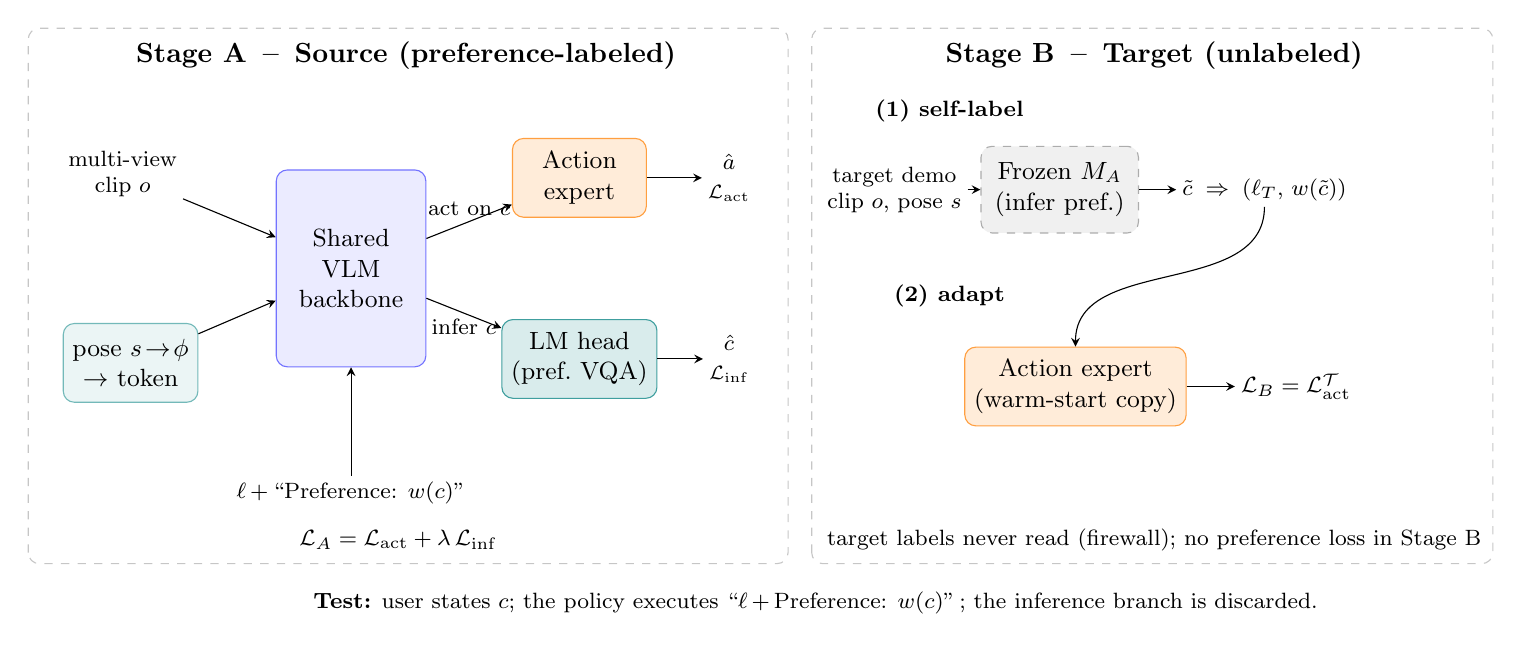
\begin{tikzpicture}[
    >=stealth, font=\small,
    io/.style   ={align=center, font=\footnotesize, inner sep=2pt},
    bb/.style   ={draw=blue!55,  fill=blue!8,   rounded corners, align=center,
                  minimum width=1.9cm, minimum height=2.5cm},
    act/.style  ={draw=orange!75, fill=orange!15, rounded corners, align=center,
                  minimum width=1.7cm, minimum height=1.0cm},
    inf/.style  ={draw=teal!75,  fill=teal!15,  rounded corners, align=center,
                  minimum width=1.7cm, minimum height=1.0cm},
    fro/.style  ={draw=gray!65,  fill=gray!12,  rounded corners, dashed, align=center,
                  minimum width=2.0cm, minimum height=1.1cm},
    ph/.style   ={draw=teal!55,  fill=teal!8,   rounded corners, align=center,
                  minimum width=1.7cm, minimum height=1.0cm},
    loss/.style ={align=center, font=\footnotesize\itshape},
  ]
  % --- panels ---
  \draw[gray!45, dashed, rounded corners] (-1.7,-3.75) rectangle (7.95,3.05);
  \draw[gray!45, dashed, rounded corners] (8.25,-3.75) rectangle (16.9,3.05);
  \node[font=\bfseries] at (3.1,2.7)  {Stage A \,--\, Source (preference-labeled)};
  \node[font=\bfseries] at (12.6,2.7) {Stage B \,--\, Target (unlabeled)};

  % --- Stage A ---
  \node[bb] (bbA) at (2.4,0) {Shared\\VLM\\backbone};
  \node[io] (obsA) at (-0.5,1.2) {multi-view\\clip $o$};
  \node[ph] (phiA) at (-0.4,-1.2) {pose $s\!\to\!\phi$\\$\to$ token};
  \node[io] (promptA) at (2.4,-2.85) {$\ell\,+\,$``Preference: $w(c)$''};
  \draw[->] (obsA) -- (bbA);
  \draw[->] (phiA) -- (bbA);
  \draw[->] (promptA) -- (bbA);
  \node[act] (actA) at (5.3,1.15)  {Action\\expert};
  \node[inf] (infA) at (5.3,-1.15) {LM head\\(pref.\ VQA)};
  \draw[->] (bbA) -- (actA) node[io,midway,above]{act on $c$};
  \draw[->] (bbA) -- (infA) node[io,midway,below]{infer $c$};
  \node[io] (ahat) at (7.2,1.15)  {$\hat a$\\[1pt]\scriptsize$\mathcal{L}_{\mathrm{act}}$};
  \node[io] (chat) at (7.2,-1.15) {$\hat c$\\[1pt]\scriptsize$\mathcal{L}_{\mathrm{inf}}$};
  \draw[->] (actA) -- (ahat);
  \draw[->] (infA) -- (chat);
  \node[loss] at (3.0,-3.45) {$\mathcal{L}_A=\mathcal{L}_{\mathrm{act}}+\lambda\,\mathcal{L}_{\mathrm{inf}}$};

  % --- Stage B ---
  \node[io, font=\footnotesize\bfseries] at (10.0,2.0) {(1) self-label};
  \node[io]  (tin) at (9.3,1.0)  {target demo\\clip $o$, pose $s$};
  \node[fro] (fro) at (11.4,1.0) {Frozen $M_A$\\(infer pref.)};
  \node[io]  (pl)  at (14.0,1.0) {$\tilde c\;\Rightarrow\;(\ell_T,\,w(\tilde c))$};
  \draw[->] (tin) -- (fro);
  \draw[->] (fro) -- (pl);
  \node[io, font=\footnotesize\bfseries] at (10.0,-0.35) {(2) adapt};
  \node[act] (s2) at (11.6,-1.5) {Action expert\\(warm-start copy)};
  \node[io]  (lb) at (14.4,-1.5) {$\mathcal{L}_B=\mathcal{L}^{\mathcal{T}}_{\mathrm{act}}$};
  \draw[->] (pl) to[out=-90,in=90] (s2);
  \draw[->] (s2) -- (lb);
  \node[io] at (12.6,-3.45)
    {target labels never read (firewall); no preference loss in Stage B};

  % --- deploy ---
  \node[io] at (8.3,-4.25)
    {\textbf{Test:} user states $c$; the policy executes ``$\ell\,+\,$Preference: $w(c)$''\,; the inference branch is discarded.};
\end{tikzpicture}
\end{document}
